\documentclass[a4paper,12pt]{article}

% defining margin for the document
\usepackage[margin=1.00in]{geometry}

% these packages are used for images
\usepackage{graphicx}

\title{Problem 4: Checkstyle}
\author{Saraswati Saud \\
Student ID: 40115097}
\date{}
\begin{document}
\maketitle
\section{Description}
    I have used the Eclipse plugin - Checkstyle Plug-in 8.44.0 to check the quality of my source code. It is a development tool that helps programmers to write Java code that follows good programming standards. It helps to improve the quality, readability, re-usability of the code and may reduce the development cost.\\
    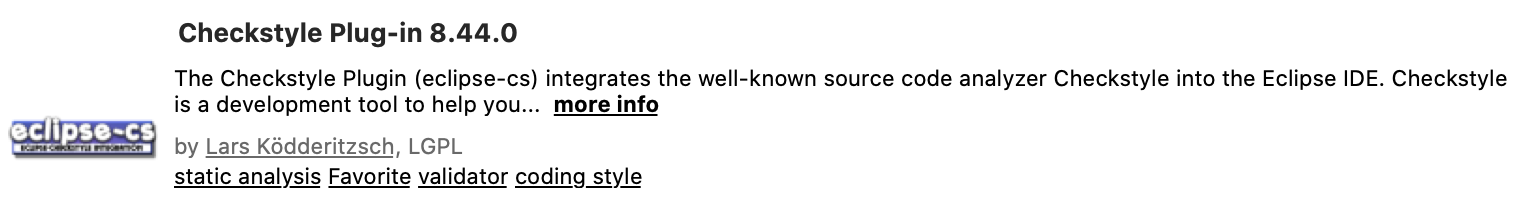
\includegraphics[width=16cm, height=4cm]{check_style.png}
    \subsection{Advantages}
    \begin{itemize}
        \item It is portable between IDEs.
        \item It is easier to integrate with external tools as it was designed as a standalone framework.
        \item It has an ability of creating own rules. Eclipse has a large set of styles but checkstyle has more and we can add our own custom rules.
    \end{itemize}
    
    \subsection{Disadvantages}
    \begin{itemize}
        \item Checkstyle is limited to a single file static analysis tool.
        \item It is also limited to the presentation of the code and hence does not confirm the correctness or completeness of the code.
    \end{itemize}
\end{document}
